\documentclass[a4paper, 12pt]{article}
\usepackage[UTF8]{ctex}
\usepackage{graphicx}

\begin{document}
	\title{第二次实验报告}   %题目
	\author{时伟杰}     %作者姓名
	\date{2024年8月30日}      %日期
	\maketitle    %制作开头
	\tableofcontents         %目录
	\newpage          %新建一页
	\pagenumbering{arabic}  %用阿拉伯数字
	\section{shell简介}         %介绍
	‌‌Shell‌是一个‌命令解释器,它在操作系统的最外层负责直接与用户对话,把用户的输入解释给操作系统,并且处理操作系统的输出结果,输出到屏幕返回给用户。这种对话方式可以是交互的方式。Shell是用‌C语言编写的程序,它是用户使用‌Linux的桥梁。Shell既是一种命令语言,又是一种程序设计语言。简单来说,Shell是指一种应用程序,这个应用程序提供了一个界面,用户通过这个界面访问操作系统内核的服务。也可以这样认为,Linux中的shell就是Linux内核的一个外层保护工具,并负责完成用户与内核之间的交互。Shell脚本是一种专门使用shell编写的脚本程序。Shell脚本编程如同其他编程语言一样,只要有一个能编写代码的文本编辑器和一个能解释执行的脚本解释器就可以运行了。其中,Bash(Bourne Again Shell)因为其能提供环境变量、支持历史记录、内置算数功能、支持通配符表达式等高效性能,被广泛应用于Debian系列的Linux发行版中。‌
	\section{vim简介}
	‌Vim‌是一个高度可定制的文本编辑器,它是Vi编辑器的改进版,增加了许多特性并提高了易用性。Vim在各种操作系统上运行,包括Linux、macOS、Windows等,这使得它成为跨平台的文本编辑器。Vim支持多种字符集和语言,包括UTF-8和Unicode,并且提供了丰富的编辑功能,如搜索和替换、宏录制与回放、多光标编辑等,这些功能有助于高效地编辑和处理各种文本文件。Vim的设计理念是减少对鼠标的依赖,通过高效的键盘操作来提高工作效率。它拥有多种模式,包括普通模式、插入模式和可视模式等,每种模式下都可以进行特定的操作,这使得Vim的使用非常灵活且功能强大。Vim的高度可定制性是其另一个重要特点,用户可以根据自己的需要配置Vim,通过修改配置文件或安装插件来扩展其功能,满足不同的编程环境和需求。此外,Vim还拥有一个庞大且活跃的社区,提供了丰富的资源和支持,无论是教程、插件还是问题解答,用户都可以轻松找到所需的帮助。这种社区支持对于学习和使用Vim的用户来说是非常宝贵的资源。
     
	\section{实例演示与截图}      %方法
	
	\begin{tabular}{|c|c|c|}   %表格
		\hline
	   shell操作 &实例       & 介绍    \\
		\hline
		1  & date   &   输出现在的日期   \\
		\hline
		2  & echo hello &    输出hello字符串  \\
		\hline
		3  & which echo &确定某个程序名代表的是哪个具体的程序\\
		\hline
		4  & pwd &    获取当前工作目录 \\
		\hline
		5  & cd /bin  & 切换到bin目录 \\
		\hline
		6  & cd .. & 切换到上级目录 \\
		\hline
		7  & ../bin/echo hello   & 另一种输出hello的方式 \\
		\hline
		8 & ls & 查看指定目录下包含哪些文件 \\
		\hline
		9 & echo debug > debug.txt   & 将dubug输入文本文档 \\
		\hline
		10 & cat debug.txt & 输入文档中内容 \\
		\hline
		11 & cat < debug.txt & 另一种输出的方式 \\
		\hline
		12 & cat < debug.txt >debug2.txt&将debug.txt中的文字输出到debug2.txt \\
		\hline
    	13 & foo=bar echo "\$foo" echo '\$foo'&单引号与双引号的区别\\
		\hline
		14 & 与、或的实例 & 与操作符、或操作符  \\
		\hline
		
		vim操作 & 实例   &   介绍   \\
		\hline
		15 & vim+文件路径 & 打开指定文件 \\
		\hline
		16 & wq & 退出文件 \\
		\hline
		17 & h或左方向键 & 光标向左移动一个字符 \\
		\hline
		18 & l或右方向键 & 光标向右移动一个字符 \\
		\hline
		19 & k或上方向键 & 光标向上移动一个字符 \\
		\hline
		20 & j或下方向键 & 光标向下移动一个字符 \\
		\hline
		21 & 0或Ctrl+6或 ome键 & 光标移动到行首 \\
		\hline
		22 & Ctrl+4或end键 & 光标移动到行尾 \\
		\hline
		23 & Ctrl+f & 屏幕向下移动一页 \\
		\hline
		24 & Ctrl+b & 屏幕向上移动一页 \\
		\hline
		25 & gg & 移动到文件的第一行 \\
		\hline
		26 & G & 移动到文件的最后一行 \\
		\hline
		27 & x   & 删除后一个字符 \\
		\hline
		28 & X & 删除前一个字符 \\
		\hline
     	\end{tabular}
     	
		\begin{tabular}{|c|c|c|}
		\hline
		vim操作 & 实例   & 介绍 \\
		\hline
		29 & dd   & 剪切一行 \\
		\hline
		30 & 数字dd   &   剪切多行   \\
		\hline
		31 & yy & 复制一行 \\
		\hline
		32 & 数字yy & 复制多行 \\
		\hline
		33 & p   & 粘贴到下一行 \\
		\hline
		34 & P & 粘贴到上一行 \\
		\hline
		35 & u   & 撤回操作 \\
		\hline
		36 & Ctrl + r   &  撤回刚才的撤回操作   \\
		\hline
		37 & i & 输入模式,进入后显示,INSTER \\
		\hline
		38& o & 输入模式,在光标下一行插入新行,INSTER\\
		\hline
		39 & R &取代模式,输入的值会取代光标所在的内容,REPLACE\\
		\hline
		40 & esc键  & 退出编辑模式(输入模式) \\
		\hline
	\end{tabular}
	\begin{figure}[h!]
		\centering
		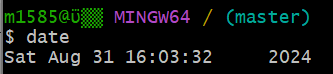
\includegraphics[width=1\textwidth]{1}
		\caption{第一个实例演示}
		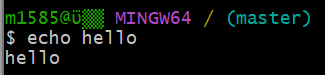
\includegraphics[width=1\textwidth]{2}
		\caption{第二个实例演示}
		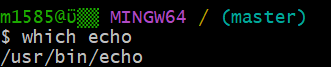
\includegraphics[width=1\textwidth]{3}
		\caption{第三个实例演示}
		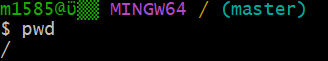
\includegraphics[width=1\textwidth]{4}
		\caption{第四个实例演示}
		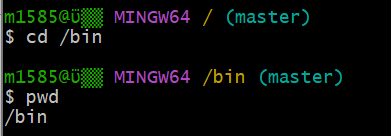
\includegraphics[width=1\textwidth]{5}
		\caption{第五个实例演示}
	\end{figure}
	\begin{figure}[h!]
		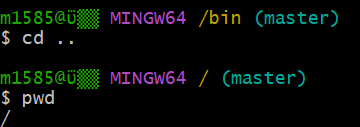
\includegraphics[width=1\textwidth]{6}
		\caption{第六个实例演示}
		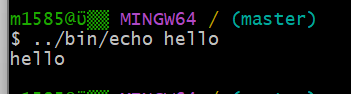
\includegraphics[width=1\textwidth]{7}
		\caption{第七个实例演示}
		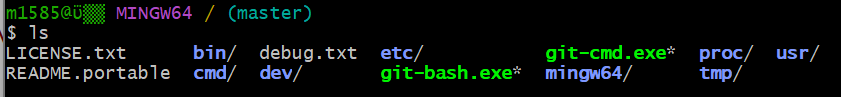
\includegraphics[width=1\textwidth]{8}
		\caption{第八个实例演示}
		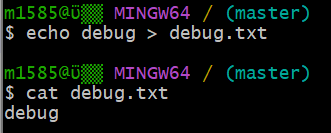
\includegraphics[width=1\textwidth]{9}
		\caption{第九、十个实例演示}
		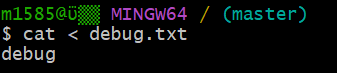
\includegraphics[width=1\textwidth]{10}
		\caption{第十一个实例演示}
	\end{figure}
	\begin{figure}[h!]
		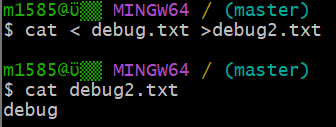
\includegraphics[width=1\textwidth]{12}
		\caption{第十二个实例演示}
		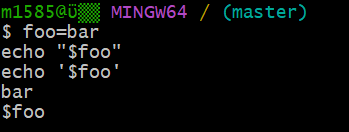
\includegraphics[width=1\textwidth]{13}
		\caption{第十三个实例演示}
		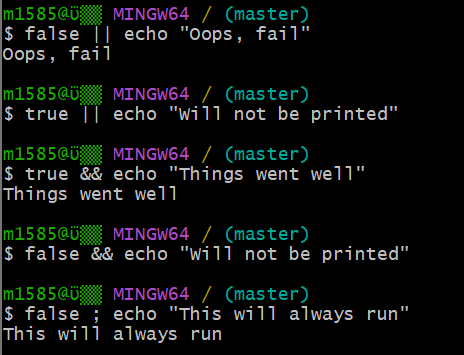
\includegraphics[width=1\textwidth]{14}
		\caption{第十四个实例演示}
	\end{figure}
    \section{心得体会}
    经过老师和助教的帮助,以及配套资料和B站视频的学习,我对shell和vim有了初步的了解,明白了学习Shell脚本让我能够高效地自动化重复性任务,比如文件处理、系统监控和数据备份。通过掌握变量、条件语句和函数,我能够编写出更灵活和复杂的脚本,提高了工作效率。同时,Vim的学习改变了我对文本编辑的理解。其模式化编辑方式虽然初看复杂,但极大提升了编辑速度。通过使用快捷键和命令,我能更快速地进行文本操作,而插件系统进一步增强了Vim的功能,使得编辑过程更加顺畅。但是学习过程是一波三折的,比如虚拟机的安装和了解更是消耗了不少时间,这也锻炼了我学习的能力和对计算机的进一步了解,综合这两者的使用,我的开发和系统管理能力得到了显著提升,使得面对各种任务时更加得心应手。
	
	
	\section{附带图片}


\end{document}
